\documentclass[aspectratio=169]{beamer}
\graphicspath{{gfx/}}

\usepackage{ragged2e}\justifying
\usepackage{txfonts}
\usepackage{booktabs}
\usepackage{natbib}
\usepackage{bibentry}
\usepackage{tikz}
\usepackage{siunitx}
\usepackage{tabularx}
\usepackage{accents} 
\usepackage{caption}

%\usepackage[hang]{footmisc}
%\setlength{\footnotemargin}{1em}

\usepackage{lipsum}

\newcommand\blfootnote[1]{%
	\begingroup
	\renewcommand\thefootnote{}\footnote{#1}%
	\addtocounter{footnote}{-1}%
	\endgroup
}
%=================================== Themes ==============================================
\usetheme{EastLansing}
 
%========================= Beamer color/font/template ==================================== 
\setbeamersize{text margin left=12mm, text margin right=12mm} 
\setbeamertemplate{frametitle}[default][left, leftskip=5mm] 
\setbeamertemplate{frametitle continuation}{\frametitle{References}}
\setbeamertemplate{bibliography item}[text] 
\setbeamertemplate{page number in head/foot}[appendixframenumber]

%=================================== Others ==============================================
\setlength{\parskip}{5pt}

\let\oldbib\bibentry
\renewcommand{\bibentry}[1]{{\tiny[\oldbib{#1}]}}

%=============================== Title information ======================================
\title[17. Symposium Energieinnovation 2022]{Designing a model for the cost-optimal decommissioning and refurbishment investment decision of gas networks}
\subtitle{CANCEL}
\author[Zwickl-Bernhard]{Sebastian Zwickl-Bernhard\\ \tiny  zwickl@eeg.tuwien.ac.at\\[5mm] 
\includegraphics[scale=0.2]{EEG}}

\institute[EEG]{Energy Economics Group (EEG),\\ Institute of Energy Systems and Electrical Drives \\ Technische Universität Wien}

\date[\tiny \today]{\scriptsize \today}

% \titlegraphic{\includegraphics[scale=0.08]{logo}}
% \logo{\includegraphics[scale=0.04]{logo}}

%=================================== Main body========================================
\begin{document}

%% References	
\bibliographystyle{APA-noTitle}
\nobibliography{mybib}	

%% Title frame	
\begin{frame}[plain, noframenumbering]
\maketitle
\begin{tikzpicture}[remember picture, overlay]
	\node[right] at (current page.207.5) 
	{
		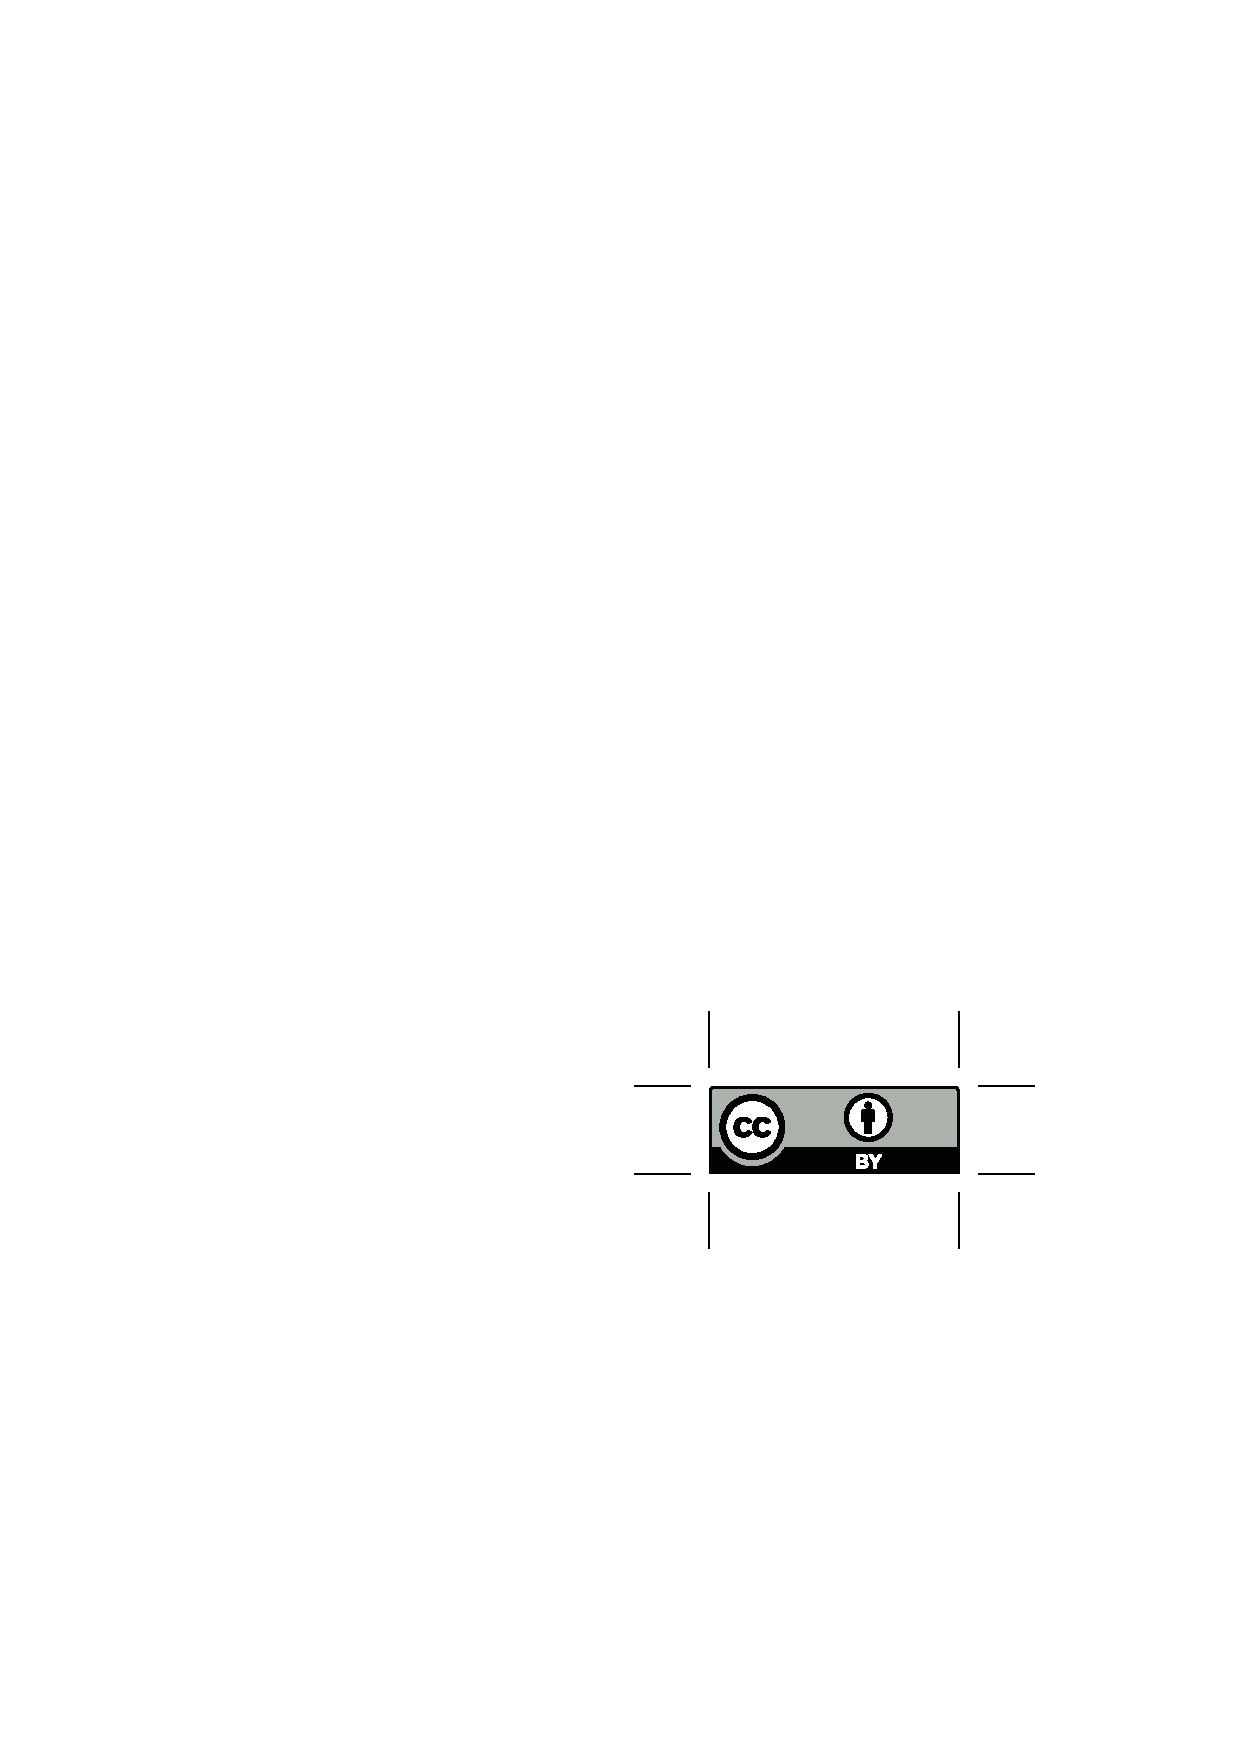
\includegraphics[scale=0.3]{by}		
	};
\end{tikzpicture}

\end{frame}	


\section[]{}
\begin{frame}{Outline}
\tableofcontents	
\end{frame}

\section{Background and motivation}
\begin{frame}[t]{Current situation of (natural) gas in Austria}
	\begin{columns}[T]
		\column{0.7\linewidth}	
		\begin{itemize}
			\item  Area-wide transmission and distribution network infrastructure ($\approx \SI{46000}{km}$)
			\item Supply of 1,245,000 households and 103,000 companies (incl. industry)
			\item Important transmission route from east (i.e., gas import) to west (i.e., gas export) and seasonal gas storage
			\item Defossilization and related (natural) gas demand reduction in line with Austrian and European decarbonization pathways
		\end{itemize}
		\column{0.3\linewidth}
	\begin{tikzpicture}[remember picture, overlay]
		\node[left] at (current page.0) 
		{
				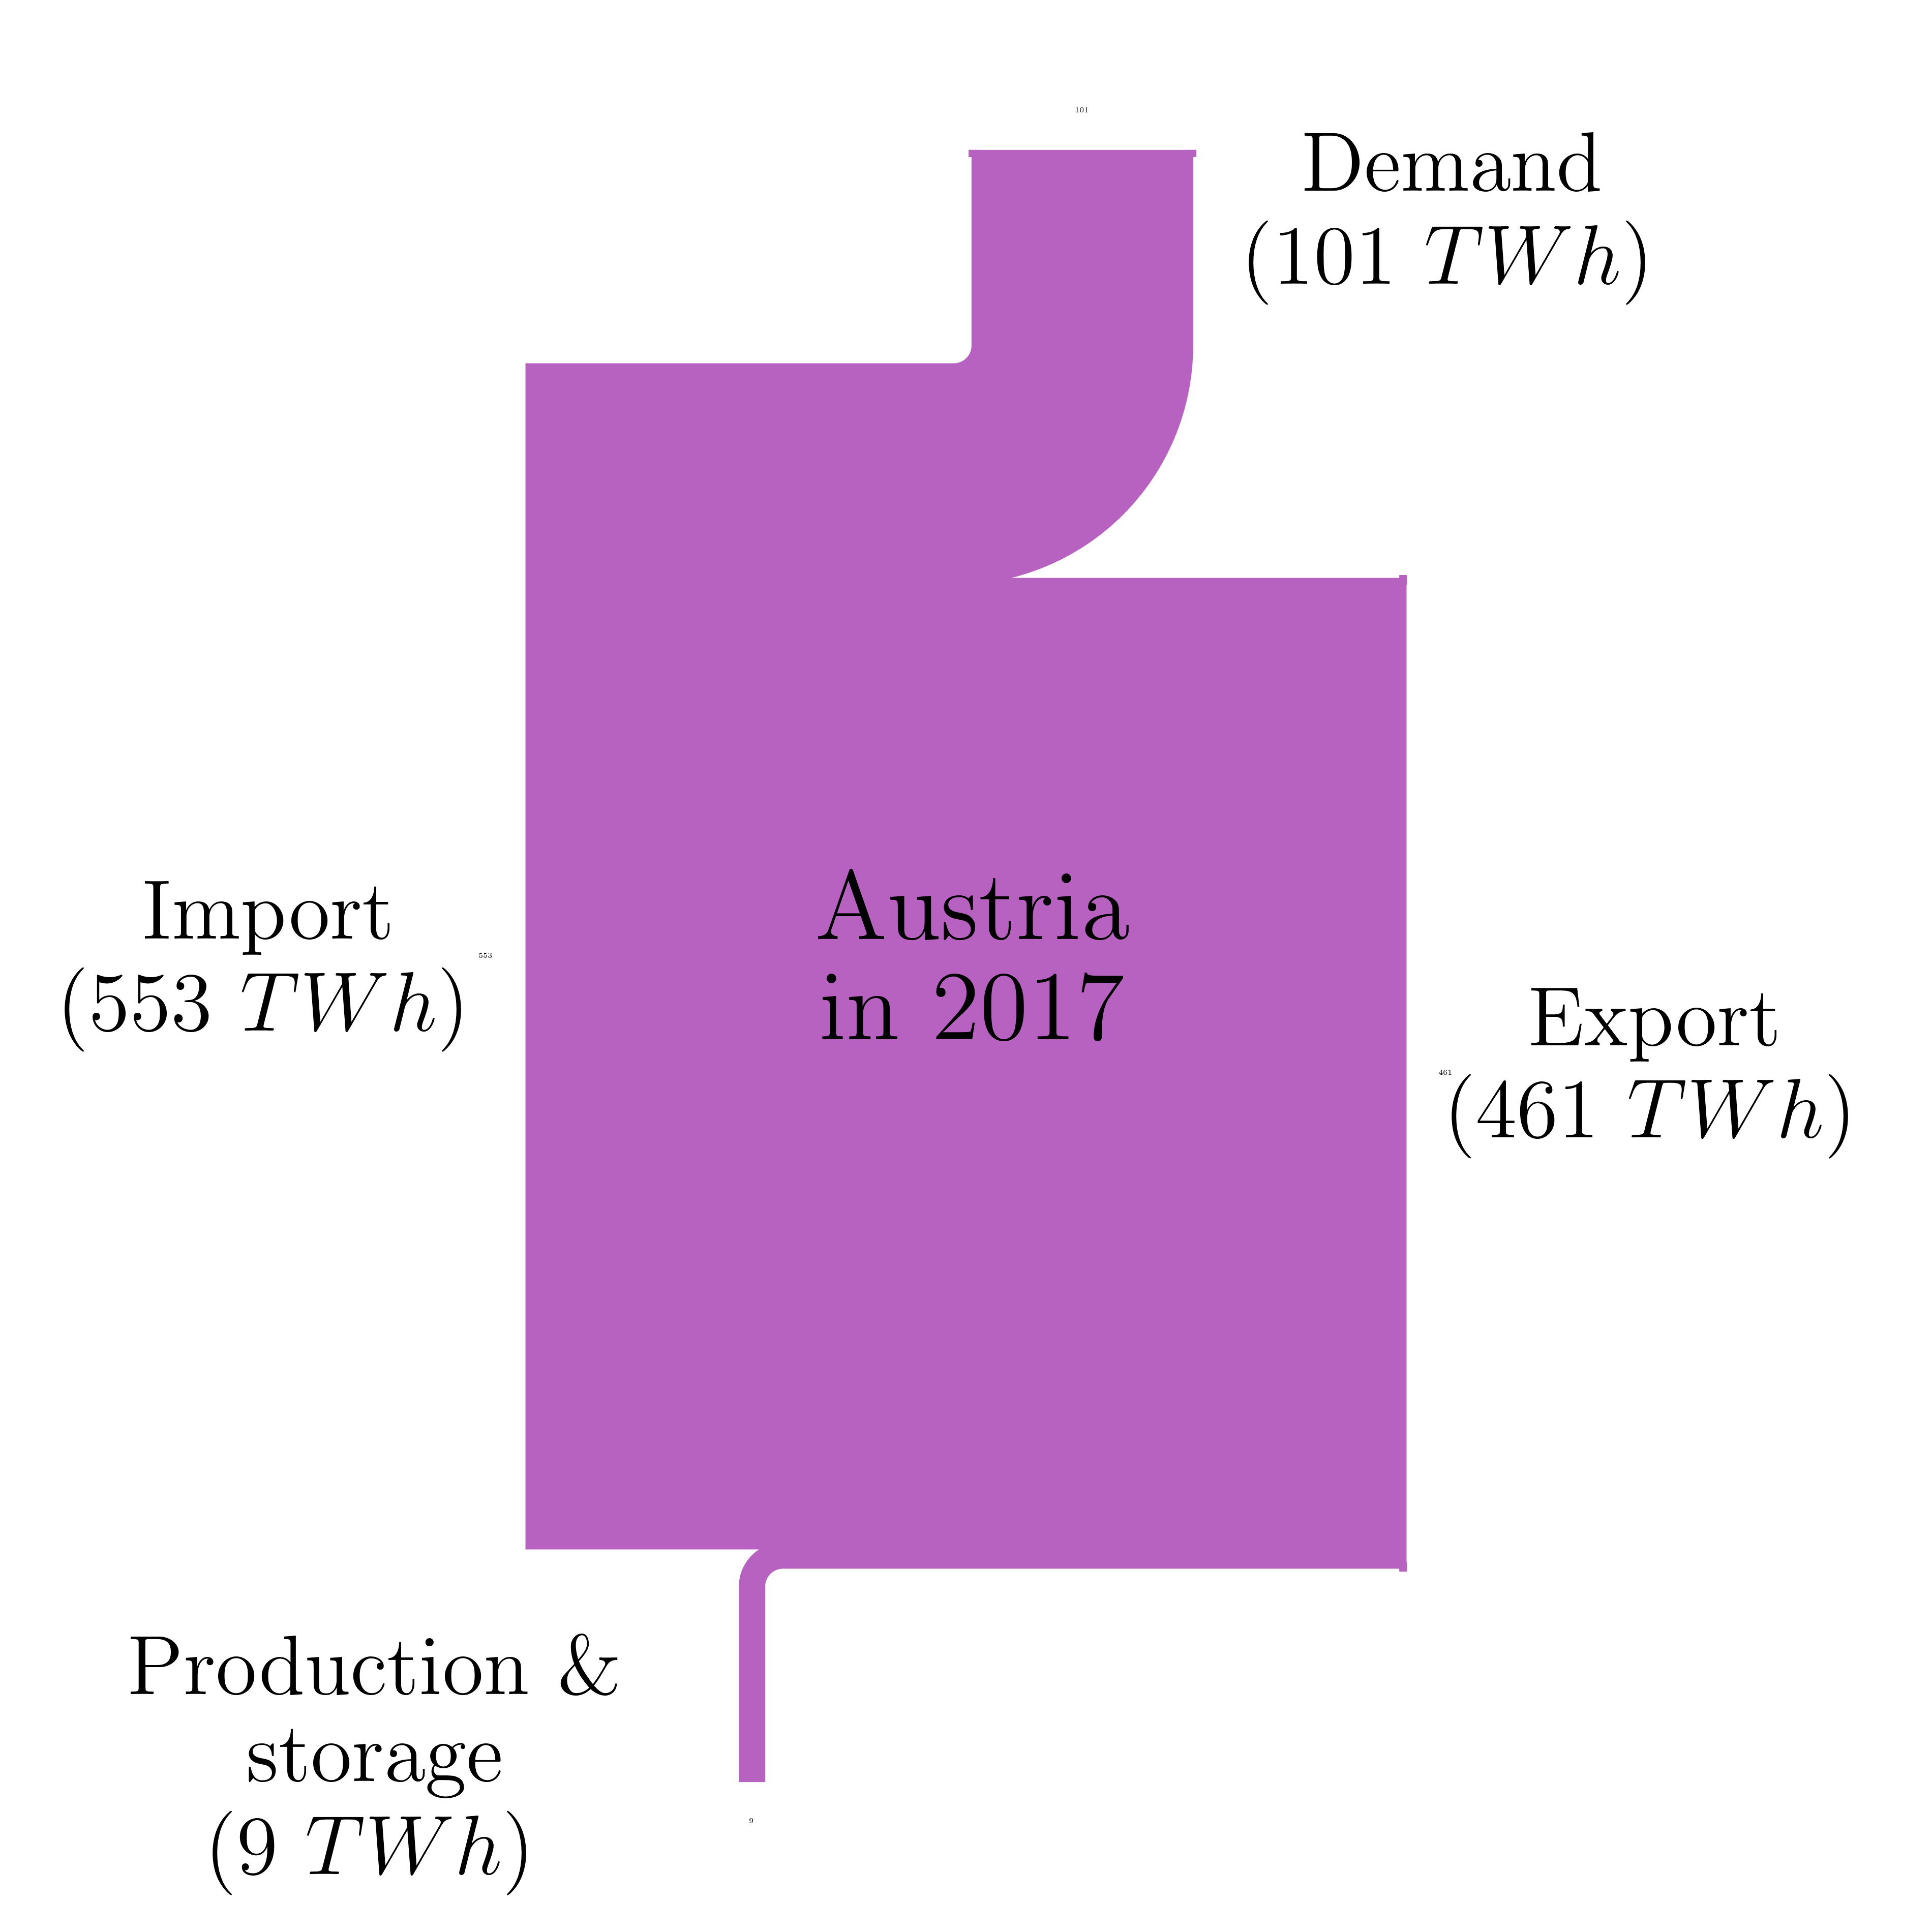
\includegraphics[scale=0.55]{Balance}
		};
	\end{tikzpicture}
	\end{columns}
\blfootnote{\tiny Holzmann, A. \& Strimitzer, L. (2019) \emph{Netzeinspeisung von erneuerbarem Gas}.}
\end{frame}






\begin{frame}[t]{Consensus between science and policymakers on natural gas}
\small"Our results suggest that, globally, a third of oil reserves, \textbf{half of gas reserves} and over 80 per cent of current coal reserves \textbf{should remain unused} from 2010 to 2050 in order to meet the target of 2.0°C." McGlade, C. \& Ekins, P. (2015) \emph{Nature 517(7533), 187-190.}
\vspace{0.25cm}
	\begin{columns}[T] 	
		\column{0.5\linewidth}	
		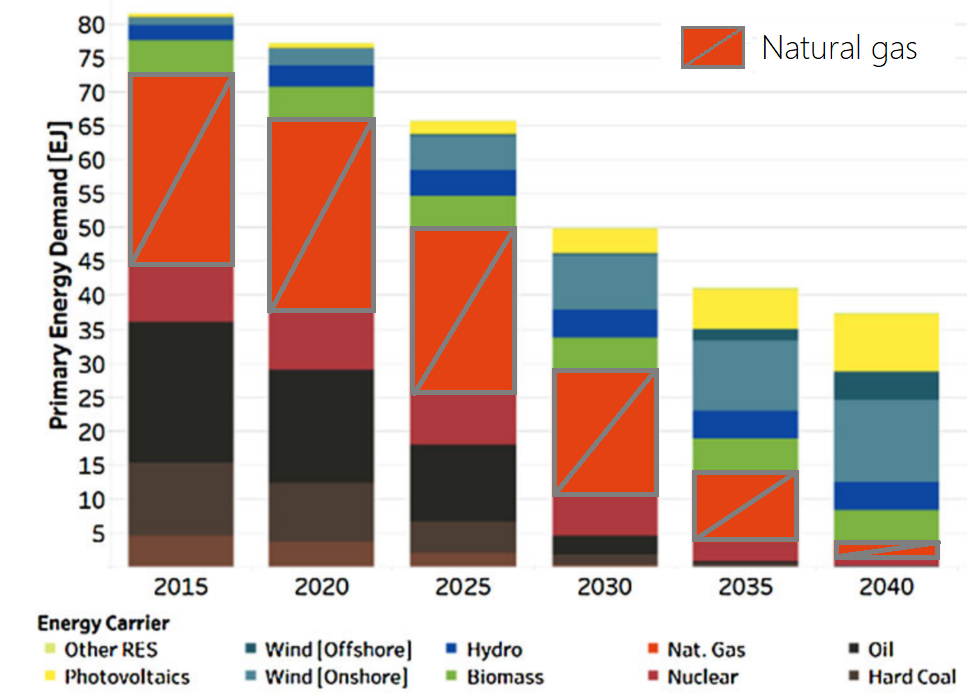
\includegraphics[width=0.8\textwidth] {openENTRANCE}\\\vspace{0.1cm}\tiny \hspace{0.75cm}Source: Auer et al. (2020) \emph{e\&i, 137(7), 346-358.}
		\column{0.5\linewidth}
		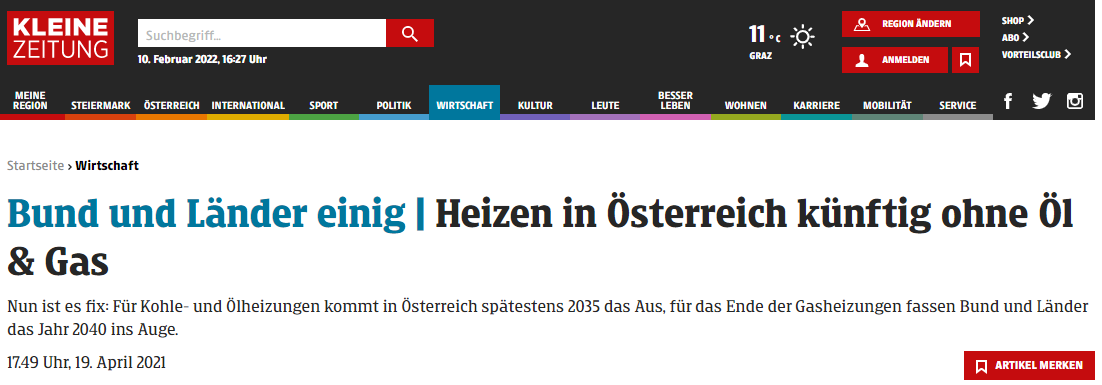
\includegraphics[width=0.85\textwidth] {policymakers}\\
		\hspace{1.75cm}\tiny(top) \href{https://www.kleinezeitung.at/wirtschaft/5968089/Bund-und-Laender-einig_Heizen-in-Oesterreich-kuenftig-ohne-Oel-Gas}{Kleine Zeitung}; (bottom) \href{https://www.ebp.ch/de/projekte/die-zukunft-der-gas-infrastruktur-im-metropolitanraum-zuerich}{EBP}\\
		\vspace{0.1cm}
		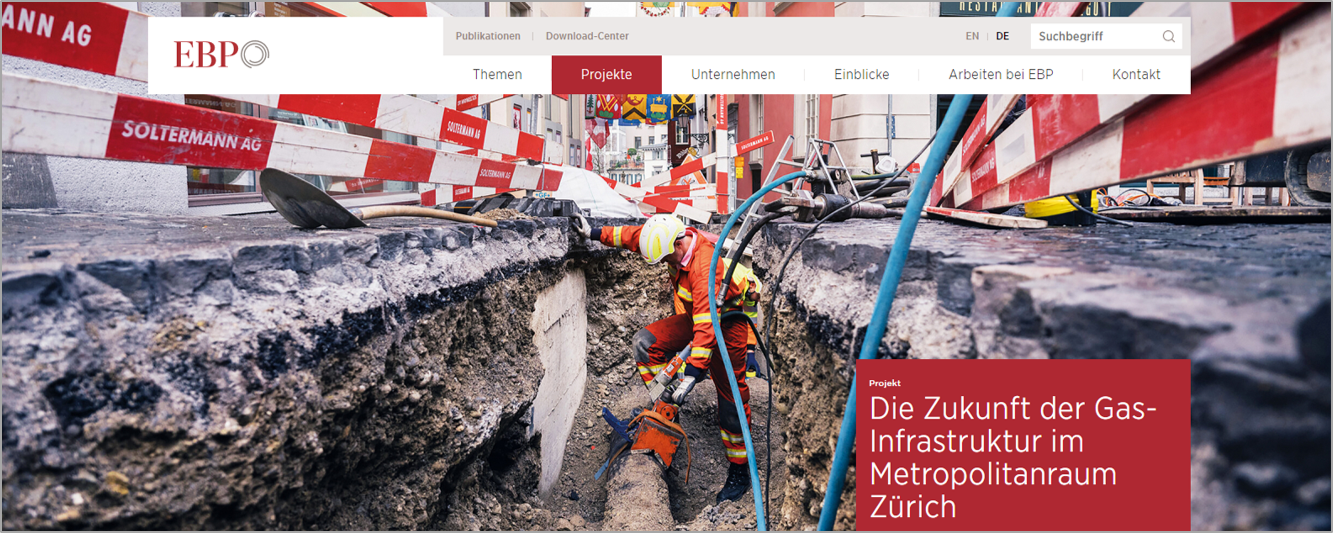
\includegraphics[width=0.85\textwidth] {zuerich}
	\end{columns} 
\end{frame}


\begin{frame}[t]{Reliability of gas supply against the risk of stranded assets}
	\vspace{-1cm}
	\begin{figure}
		\centering
		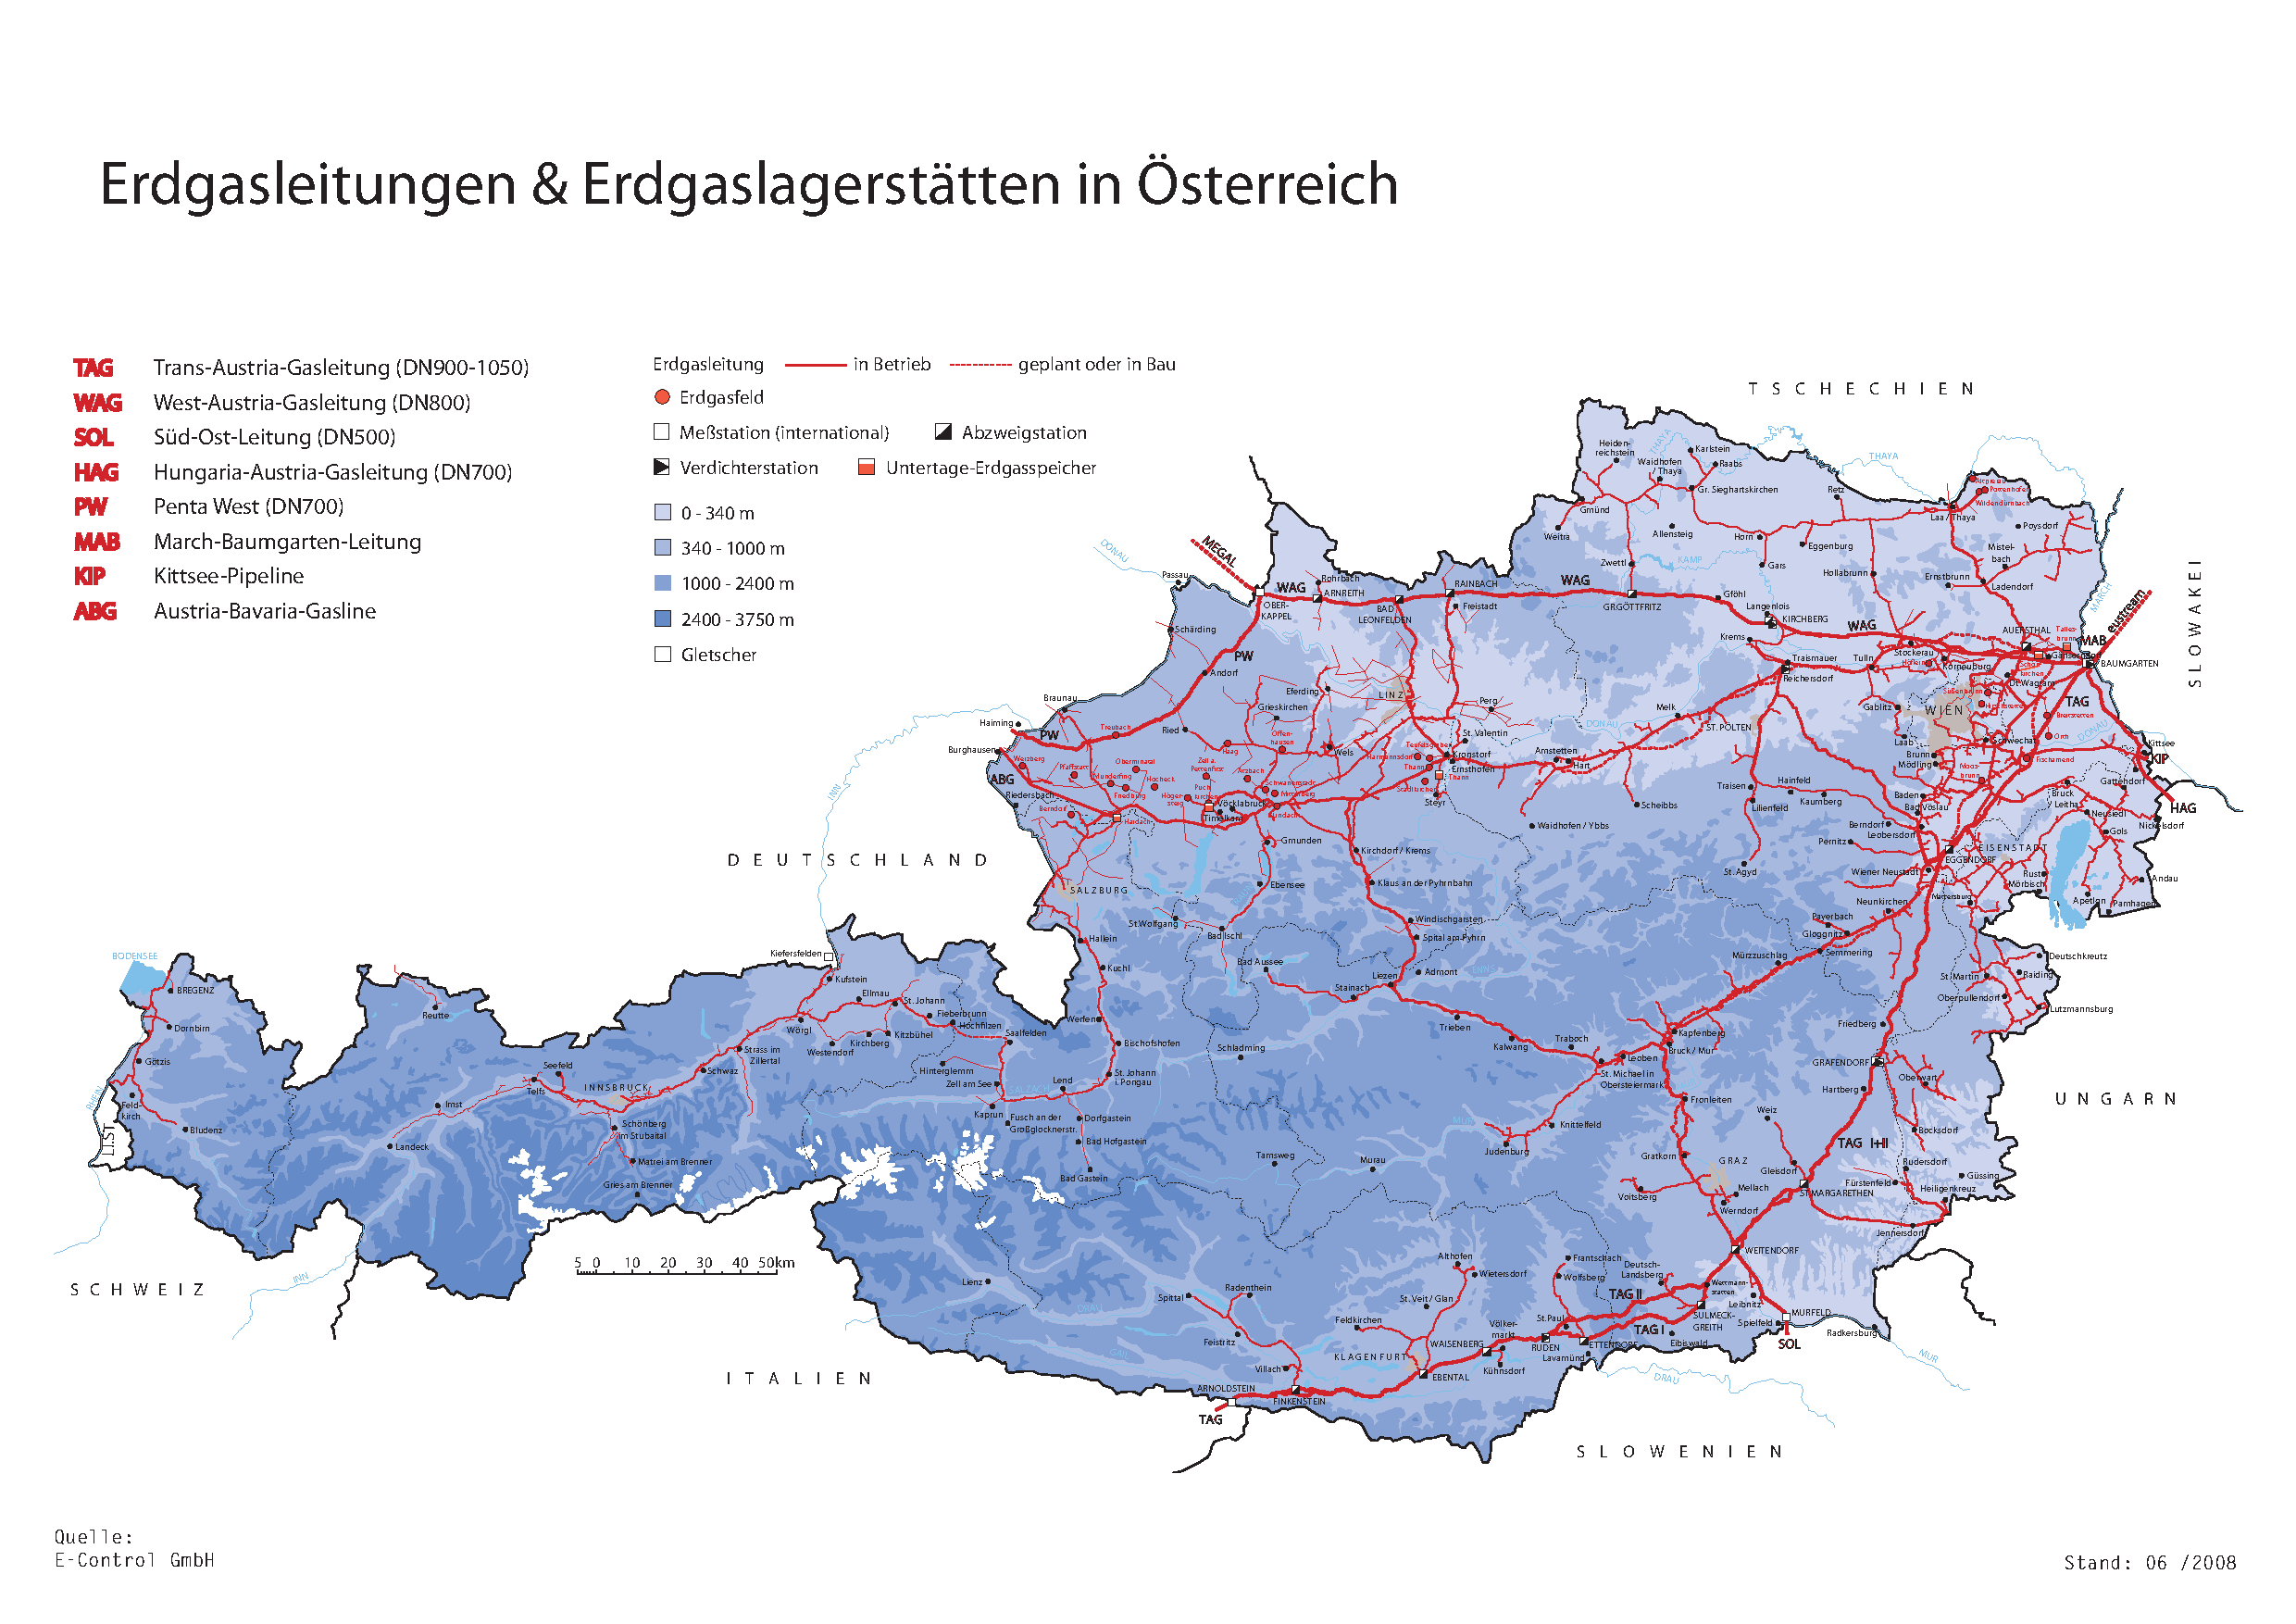
\includegraphics[scale=0.25]{gas_network}
		\vspace*{-1\textheight}
	\end{figure}
 \centering\vfill
 \vspace{2cm}
 \fontsize{40}{72}\selectfont\color{black}\rotatebox{30}{2050?}
 \vfill 
\end{frame}


\section[]{Main research question and core objective}
\begin{frame}[t]{This work's scope (system analysis)}
	\begin{block}{Main research question:}
		\begin{itemize}
			\item  How does the cost-effective transmission and distribution gas network in Austria until 2050 look like?
			\item What impact does the expected decline in gas demand as a result of the defossilization of the provision of energy services have on the decision of decommissioning and refurbishment investments of gas pipelines at the local levels in Austria?
		\end{itemize}		 
	\end{block}

	\begin{block}{Core objective:}
		\begin{itemize}
			\item  The cost-effective development of the existing gas networks (incl. transmission and distribution network levels) in Austria until 2050.
			\item  In particular, the development encompasses the decision of decommissioning and refurbishment investments of gas pipelines at the community level.
		\end{itemize}		 
	\end{block}
\end{frame}
	
	
%\scriptsize
%\begin{enumerate}
%	\item  Item One
%	\item  Item Two
%	\item  Item Three
%	\item  Item Four
%\end{enumerate}

\section[Methodology]{Methodology}
\begin{frame}[t]{Overview of the modeling framework}
		\vspace{-0.3cm}
	\begin{figure}
		\centering
		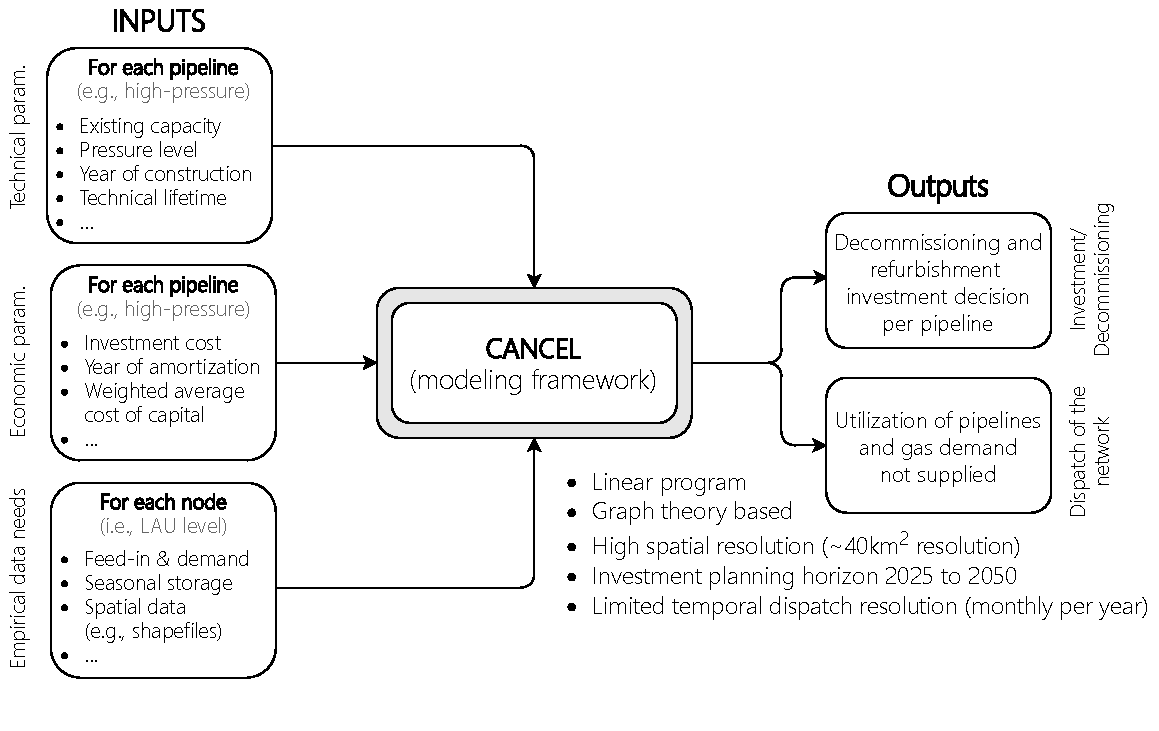
\includegraphics[scale=0.55]{flowchart}
	\end{figure}
\end{frame}

\begin{frame}{Mathematical formulation (1/3)}
	\begin{center}
		\vspace{-0.75cm}
		\renewcommand{\arraystretch}{1.}
		\centering
		\small
		\begin{tabular}{lm{7.75cm}r}
			Type & Description & Unit\\
			\hline
			Set and Index & & \\
			\hline
			{$p \in \mathcal{P}=\{1,\ldots,P\}$} & Pipeline for gas transport, index by $p$\\
			{$n \in \mathcal{N}=\{1,\ldots,N\}$} & Node of the gas network, index by $n$\\
			{$l \in \mathcal{L}=\{1,\ldots,L\}$} & Gas network level (e.g., high-pressure), index by $l$\\
			{$y \in \mathcal{Y}=\{1,\ldots,Y\}$} & Years, index by $y$\\
			{$m \in \mathcal{M}=\{1,\ldots,M\}$} & Months, index by $m$\\
			\hline
			\multicolumn{2}{l}{Decision Variables (Selection)}\\
			\hline
			{$Capex$} & Capital expenditures & \SI{}{EUR}\\
			{$Opex$} & Operational expenditures & \SI{}{EUR}\\
			{$Revenues$} & Revenues generated by gas supply & \SI{}{EUR}\\
			{$\gamma_{p,l,y}$} & Capacity of pipeline $p$ at $l$ in $y$& \SI{}{MW}, \SI{}{GW}\\
			{$q^{dem}_{n,l,y,m}$} & Gas demand supplied at $n$ and $l$ in $y$ and $m$ & \SI{}{MWh}, \SI{}{GWh}\\
			{$q_{p,l,y,m}$} & Quantity of gas transported at $p$ and $l$ in $y$ and $m$& \SI{}{MW}, \SI{}{GW}\\
			{$\Pi_{p,l,y}$} & Book value of pipeline $p$ at $l$ in $y$ & \SI{}{EUR}\\
			\hline
		\end{tabular}
	\end{center}
\end{frame}

\begin{frame}{Mathematical formulation (2/3)}
	\begin{center}
		\vspace{-0.75cm}
		\renewcommand{\arraystretch}{1.2}
		\centering
		\small
		\begin{tabular}{lm{7.75cm}r}
			Type & Description & Unit\\
			\hline
			\multicolumn{2}{l}{Parameters (Selection)}\\
			\hline
			{$\gamma^{pre}_{p,l,y}$} & Pre-existing capacity of pipeline $p$ at $l$ in $y$ & \SI{}{MW}, \SI{}{GW}\\
			{$d^{max}_{n,l,y,m}$} & Maximum gas demand at $n$ and $l$ in $y$ and $m$ & \SI{}{MWh}, \SI{}{GWh}\\
			{$q^{fed}_{n,l,y,m}$} & Quantity of gas fed at $n$ and $l$ in $y$ and $m$ & \SI{}{MW}, \SI{}{GW}\\
			{$c^{inv}_{l}$} & Specific refurbishment investment costs at $l$  & \SI{}{EUR \per MW \per km}\\
			{$\Pi^{pre}_{p,l,y}$} & Book value of pre-existing pipeline $p$ at $n$ in $y$& \SI{}{EUR}\\
			{$y^{inv}_{p,l}$} & Year of refurbishment/decommissioning per $p$ and $l$ & \SI{1}{}\\
			{$\omega$} & Weighted average cost of capital & \SI{}{\%}\\
			{$i$} & Interest rate (for calculating the net present value) & \SI{}{\%}\\
			\hline
		\end{tabular}
	\end{center}
\end{frame}

\begin{frame}{Mathematical formulation (3/3)}
	\begin{block}{Objective function:}
		$$\underset{x}{\mathrm{min~}} \left(
		\underbrace{Capex + Opex}_{\text{Assets/pipelines}} - \underbrace{Revenues}_{\text{Demand coverage}} +  \underbrace{Purchase}_{\text{Storage}}\right) $$
	\end{block}
	\begin{block}{Demand constraint:}
		$$
		\underbrace{q^{dem}_{n,l,y,m}}_{\text{Supplied}} \leq \underbrace{d^{max}_{n,l,ym}}_{\text{Total}} \quad\iff\quad \textcolor{black}{q^{dem}_{n,l,y,m}} + \textcolor{red}{\underbrace{q^{dem,not}_{n,l,y,m}}_{\text{Not supplied}}} = d^{max}_{n,l,ym}
		$$
	\end{block}
\end{frame}

\begin{frame}{Test and verification of the model by different demands and wacc}
	\begin{columns}[T] 	
		\column{0.4\linewidth}	
		\vspace{0.3cm}
		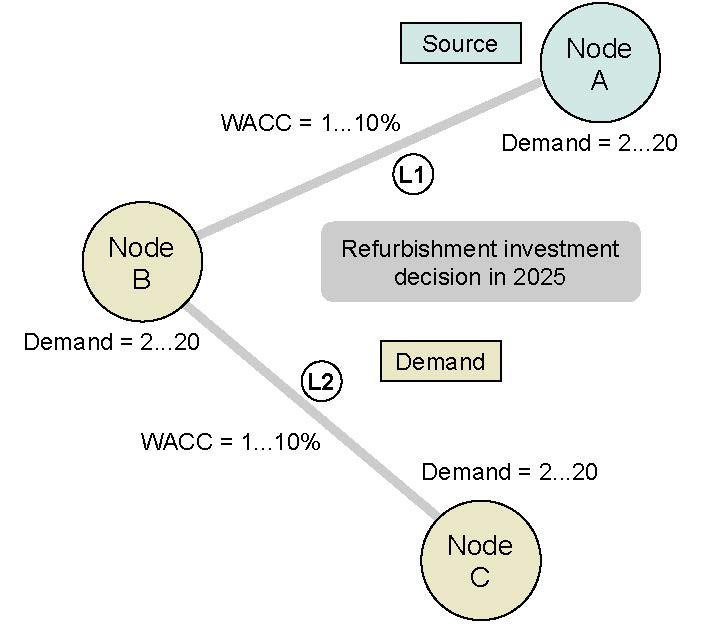
\includegraphics[scale=0.6]{FigA}\\
		\vspace{0.2cm}
		\hspace{1.5cm}\tiny (a) Simplified gas network topology
		\column{0.6\linewidth}
		\vspace{-0.1cm}
		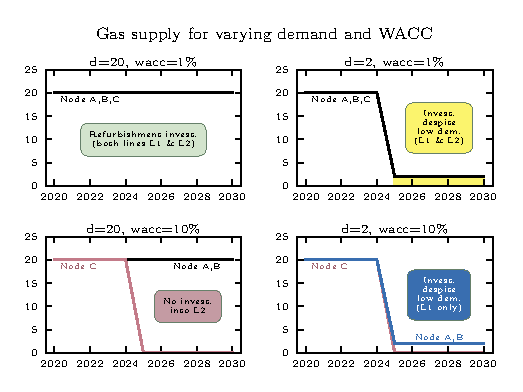
\includegraphics[scale=0.9]{results.eps}\\
		\vspace{0.2cm}
		\hspace{1.5cm}\tiny (b) Four different cases (high/low demand and wacc)
	\end{columns} 
\end{frame}

\begin{frame}{Case example: Vorarlberg's gas network until 2050}
	\begin{columns}[T] 	
		\column{0.5\linewidth}	
		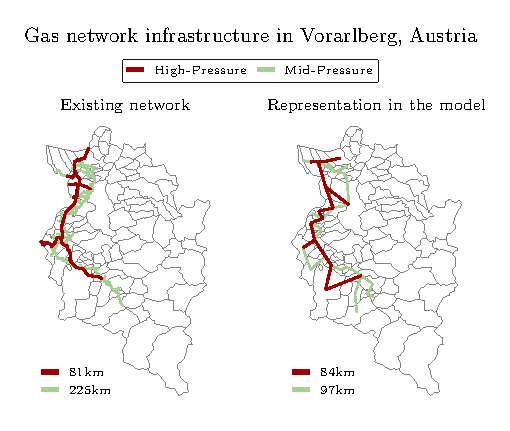
\includegraphics[scale=0.85]{Network_T8.eps}
		\column{0.5\linewidth}
		\vspace{0.75cm}
		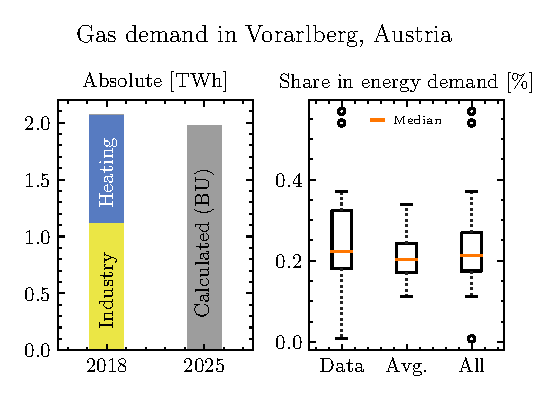
\includegraphics[scale=0.75]{Comparison_of_the_demand.eps}
	\end{columns} 
\blfootnote{\tiny Sources: \href{https://www.vorarlbergnetz.at/erdgasnetz.htm}{Vorarlberger Energienetze} and \href{https://www.energiemosaik.at/intro}{Energiemosaik Austria}}
\end{frame}


	
	
	
%	Example of a display math:
%	$$E = mc^2$$ 
%	\scriptsize
%	

%	
%	\begin{columns}[T]
%		\column{0.4\linewidth}
%		\begin{itemize} 
%			\item $v_d = -\frac{k_BT}{6\pi\mu(x_0)^2a}m\left(\frac{\mathrm{d}C(x_0)}{\mathrm{d}x}\right)$
%			\item $\frac{\mathrm{d}C(x_0)}{\mathrm{d}x} \approx \frac{\Delta C(x_0)}{\sigma}$
%			\item $m$ = $5.4\times 10^{-5}$ Pa-s
%			\item  $\eta(x_0) = 0.85-0.88 \ \text{cP},$ 
%			$k_B=1.38\times 10^{-23}$, $T=300$ K, $\sigma = 2a = 200 \ \text{nm}$
%			\item for $c=0.5\%$, $v_d \approx 4\times10^{-9}$ m/s 
%		\end{itemize}
%		
%		\column{0.5\linewidth}
%		\includegraphics[width=0.75\linewidth]{drift-speed}	
%	
%	\end{columns}	

	
	
	
%	\scriptsize	
%\begin{columns}[t]
%\column{0.32\linewidth}	
%	\begin{enumerate}
%	\item  Item One
%	\item  Item Two
%	\item  Item Three
%	\item  Item Four
%\end{enumerate}
%
%\column{0.32\linewidth}	
%	\begin{itemize}
%	\item  Item One
%	\item  Item Two
%	\item  Item Three
%	\item  Item Four
%	\item  Item Three
%	\item  Item Four
%\end{itemize}
%
%\column{0.32\linewidth}	
%\begin{enumerate}
%	\item  Item One
%	\item  Item Two
%	\item  Item Three
%	\item  Item Four
%	\item  Item One
%	\item  Item Two
%	\item  Item Three
%	\item  Item Four
%\end{enumerate}	
%	
%\end{columns}


% \begin{frame}{Blocks}
% \scriptsize	
% \begin{columns}[t]	
% \column{0.3\linewidth}		
%\begin{block}{Title of the block}
%\begin{enumerate}
%	\item  Item One
%	\item  Item Two
%	\item  Item Three
%	\item  Item Four
%	\item  Item One
%	\item  Item Two
%	\item  Item Three
%	\item  Item Four
%\end{enumerate}		 
%\end{block}
%
%\column{0.3\linewidth}	
%\begin{exampleblock}{Title of the example block} 
%	\begin{enumerate}
%		\item  Item One
%		\item  Item Two
%		\item  Item Three
%		\item  Item Four
%		\item  Item One
%		\item  Item Two
%		\item  Item Three
%		\item  Item Four
%	\end{enumerate}	
%\end{exampleblock}
%
%\column{0.36\linewidth}	
%\begin{alertblock}{Title of alert block}
%\begin{enumerate}
%	\item  Item One
%	\item  Item Two
%	\item  Item Three
%	\item  Item Four
%	\item  Item One
%	\item  Item Two
%	\item  Item Three
%	\item  Item Four
%\end{enumerate}	
%\end{alertblock}
%                                  	
%\end{columns} 	
% \end{frame}
%
%%--------------------------------------------------------------------------
%
%%--------------------------------------------------------------------------

%\begin{frame}{Figures and Tables}
%\centering\tiny 	
%\begin{columns}[T] 	
%\column{0.32\linewidth}	
%\includegraphics[width=0.96\textwidth] {aq-suc-vis}\\ (a)
%
%\column{0.32\linewidth}
%\includegraphics[width=0.95\textwidth] {xe_mu_h}\\ (b)
%
%\column{0.32\linewidth}
%\includegraphics[width=0.95\textwidth] {drift-speed}\\ (c)	
%\end{columns} 
%
%\tiny 
%\begin{tabular}{llll}
%	\toprule
%	S. no. & Upper phase  & Lower phase &  Strings (Y/N)\\
%	\midrule
%	1& Lipid/ethanol & W & Y  \\
%	2& PS/ethanol & W & Y\\
%	3 & PS/methanol & W  & Y\\
%	4 & PS/propanol & W  & Y\\
%	5 & PS/sucrose & W & N\\
%	6 & PS/water & W  & N\\
%	\bottomrule
%\end{tabular}	
%\end{frame}




\section{Illustrative results}

\begin{frame}{}
\begin{minipage}{.3\textwidth}
\centering

\begin{tabularx}{1\linewidth}{XXX}
\toprule
Type & Decline & 2050 \\
\midrule
Res. & linearly & 0\\
Serv. & 8\% & 12\%\\
Ind. & 4\% & 36\%\\
\bottomrule
\end{tabularx}\\
\vspace{0.25cm}
\tiny (a) Gas demand development


\end{minipage}
\begin{minipage}{.75\textwidth}
\centering
\hspace{0.cm}
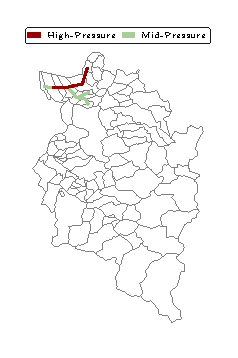
\includegraphics[width=.5\linewidth]{network.eps}
\end{minipage}
\end{frame}

%\begin{frame}{}
%	\begin{columns}[T] 	
%		\column{1\linewidth}	
%		\centering
%		\vspace{-0.1cm}
%		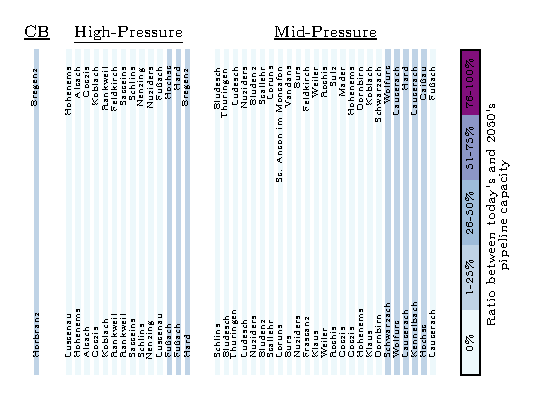
\includegraphics[width=0.82\textwidth]{Heat_Bar.eps}
%	\end{columns}
%\end{frame}
\begin{frame}{}
	\definecolor{Gray}{gray}{0.95}
	\begin{table}[h]
		\centering
		\captionsetup{font=scriptsize}
		\resizebox{1\textwidth}{!}{% use resizebox with textwidth
			\renewcommand{\arraystretch}{2}
			\begin{tabular}{cccc}
				\toprule
				\multicolumn{2}{c}{Input} & \multicolumn{2}{c}{Output}\\\cmidrule(lr){1-2}\cmidrule(lr){3-4}
				Model run & Demand constraint & Network & Result\\\hline
				1 & $q^{dem}_{n,l,y,m} \leq d^{max}_{n,l,ym}$ & Cost-optimal without ensured supply & Demand supplied $(\accentset{\ast}{\mathbf{q}}^{dem}_{n,l,y,m})$\\
				2 & $q^{dem}_{n,l,y,m} = \accentset{\ast}{\mathbf{q}}^{dem}_{n,l,y,m}$ & Cost-optimal without ensured supply (CO) & Nodal shadow price $(\lambda^{CO}_{n,l,y,m})$\\
				3 & $q^{dem}_{n,l,y,m} = d^{max}_{n,l,ym}$ & Cost-optimal with ensured supply (ES) & Nodal shadow price $(\lambda^{ES}_{n,l,y,m})$\\
		\end{tabular}}
		\caption{Model runs and related demand constraint variation used to obtain cost-optimal demand supplied and nodal shadow prices}
	\end{table}
\end{frame}

\section[]{Conclusions and future work}


\begin{frame}{Conclusions and further work}
\begin{block}{}
\begin{itemize}\setlength{\itemsep}{3mm}\footnotesize
	\item Large parts of gas network are decommissioned under assumed gas demand developments
	\item High shares of unsupplied gas demand under cost-optimality of gas networks 
	\item Detailed analysis of gas demands at the community level (incl. their energy services covered)
	\item Comparison of gas networks w/ unsupplied demand constraints
	\item Shadow prices at the nodal level (i.e., community level) provides an estimate of the costs necessary to economically substitute natural gas with alternatives
\end{itemize}
\end{block}
\end{frame}
	
\end{document}
